\documentclass{article}
\usepackage[utf8]{inputenc}
\usepackage{amsmath}
\usepackage{comment}

\title{Compton Scattering with Relativistic Electrons}
\author{T. Susai Rajan}
\date{June 2021}

\usepackage[nottoc]{tocbibind}
\usepackage{graphicx}
\usepackage{mathtools}
\usepackage{physics}
\usepackage[margin=1in]{geometry}

\usepackage{tikz}
\usetikzlibrary{arrows,shapes,positioning}
\usetikzlibrary{decorations.markings}
\tikzstyle arrowstyle=[scale=1]
\tikzstyle directed=[postaction={decorate,decoration={markings, mark=at position .5 with {\arrow[arrowstyle]{stealth}}}}]
\tikzstyle reverse directed=[postaction={decorate,decoration={markings, mark=at position .5 with {\arrowreversed[arrowstyle]{stealth};}}}]


\begin{document}

\maketitle

\tableofcontents


\section{Introduction}

Compton scattering occurs when a photon interacts with a stationary electron and imparts a portion of its kinetic energy and momentum to it. This effect is well-known and has its uses in medical imaging and radiation therapy. At the opposite end of the spectrum, the interaction of photons and relativistic electrons is common in astrophysical phenomena such as supernovae and active galactic nuclei. Low energy photons are scattered to high energies by relativistic electrons so that the photons gain and the electrons lose energy. This process is called inverse Compton scattering because the electrons lose energy rather than the photons, the opposite of the standard Compton effect. In both these effects, the particles energy and momenta are exchanged and their trajectories altered after collision as shown in Figure I.

\begin{center}
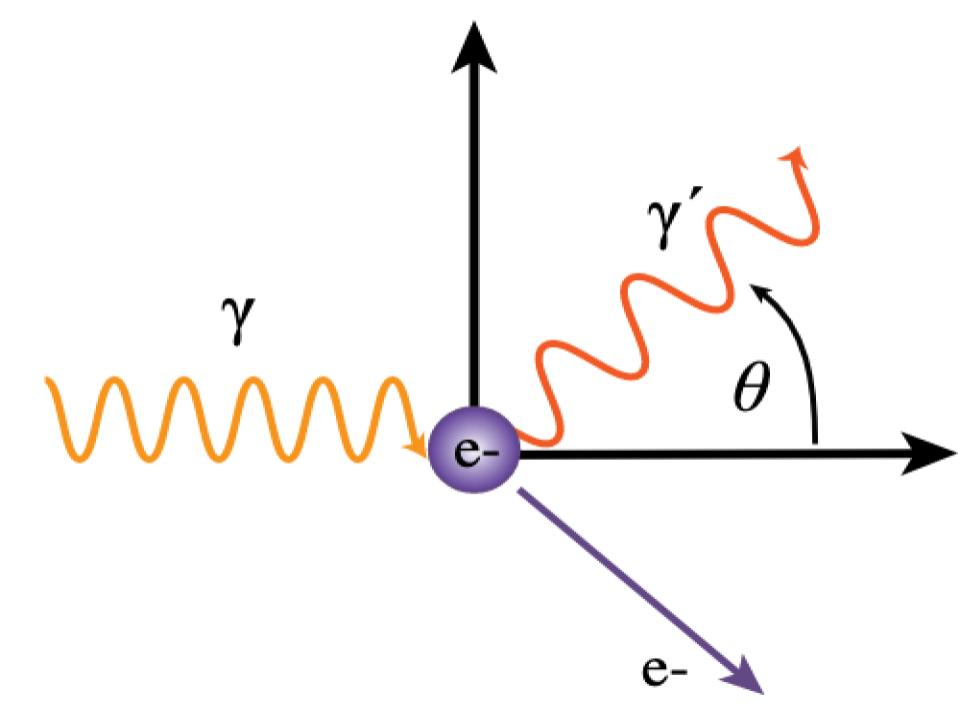
\includegraphics[width=12cm, height=9cm]{Compton_scattering.jpg} \\

Figure I. Compton scattering of a photon off of an initially stationary electron. Adapted from Reference 1.
\end{center}

\noindent The wavelength and energy of the scattered photon are given by equations (1) and (2) respectively.

\begin{align}
\Delta\lambda &= \lambda' - \lambda = \left(\dfrac{h}{m_ec}\right)(1 - \cos\theta)\\
E_{\gamma'} &= \dfrac{E_{\gamma}}{1 + \left(\dfrac{E_{\gamma}}{m_ec^2}\right)(1 - \cos\theta)}
\end{align}

In this paper, we derive equations for the energy and wavelength of a scattered photon for a more general case when the photon is collided at an arbitrary angle $\phi$ by an electron moving initially at relativistic speeds.

\section{Derivation in Lab Frame}

We start from the conservation of energy and momentum laws for the photon-electron system.

\begin{equation}
E_{\gamma} + E_{e} = E_{\gamma'} + E_{e'}
\end{equation}
\begin{equation}
\vb P_{\gamma} + \vb P_{e} = \vb P_{\gamma'} + \vb P_{e'}
\end{equation}

\begin{center}
\begin{tikzpicture}

% define coordinates
\coordinate (O) at (0,0) ;
\coordinate (A) at (0,4) ;
\coordinate (B) at (0,-4) ;
\coordinate (C) at (4,0) ;
\coordinate (D) at (-4,0) ;

% media
\fill[blue!25!,opacity=.3] (0,4) rectangle (4,-4);
\fill[blue!60!,opacity=.3] (-4,4) rectangle (0,-4);
\node[right] at (1.5,2) {After};
\node[left] at (-1.5,-2) {Before};

% axis
\draw[dash pattern=on5pt off3pt] (A) -- (B) ;
\draw[dash pattern=on5pt off3pt] (D) -- (C) ;
\draw[dash pattern=on5pt off3pt] (O) -- (-37.75:5);

% photon
\draw[ultra thick, blue, directed] plot[domain=-4*pi:0, samples=45]  (\x/pi,{0.4*sin(\x r)});
\node[] at (195:1.8)  {$\gamma$};
\draw[ultra thick, blue, directed] plot[domain=0:4*pi, samples=45]  (\x/pi,{-\x/4+0.4*sin(\x/2 r)});
\node[] at (-50:2.5)  {$\gamma'$};

% electron
\draw[black,ultra thick,reverse directed] (O) -- (150:4.6);
\draw[black,directed,ultra thick] (O) -- (10:4.05);
\node[] at (140:2.5)  {$e$};
\node[] at (24:2)  {$e'$};

% angles
\draw (-0.75,0) arc (180:150:0.75);
\draw (1.5,0) arc (0:-37.75:1.5) ;
\node[] at (-20:1.8)  {$\theta$};
\node[] at (163:1)  {$\phi$};
\end{tikzpicture}
\end{center}

\begin{center}
    Figure II. Scattering of a photon off of an initially moving electron at an angle $\phi$.
\end{center}

\noindent \\ Using the following substitutions

\begin{align*}
E_{\gamma} &= hf\\
E_{\gamma'} &= hf'\\
E_{e} &= \sqrt{(P_ec)^2 + (m_ec^2)^2}\\
E_{e'} &= \sqrt{(P_{e'}c)^2 + (m_ec^2)^2}
\end{align*}

\noindent we can rewrite (3) as

\begin{equation*}
hf + \sqrt{(P_ec)^2 + (m_ec^2)^2} = hf' + \sqrt{(P_{e'}c)^2 + (m_ec^2)^2}
\end{equation*}

\noindent which simplifies to

\begin{align*}
\begin{split}
hf - hf' + \sqrt{(P_ec)^2 + (m_ec^2)^2} &= \sqrt{(P_{e'}c)^2 + (m_ec^2)^2} \\
(hf - hf' + \sqrt{(P_ec)^2 + (m_ec^2)^2})^2 &= (P_{e'}c)^2 + (m_ec^2)^2 \\
(P_{e'}c)^2 &= (hf - hf' + \sqrt{(P_ec)^2 + (m_ec^2)^2})^2 - (m_ec^2)^2 \\
&= (hf)^2 - 2h^2ff' + 2hf\sqrt{(P_ec)^2 + (m_ec^2)^2} + (hf')^2 - \\
&\hspace{5mm} 2hf'\sqrt{(P_ec)^2 + (m_ec^2)^2} + (P_ec)^2 + (m_ec^2)^2 - (m_ec^2)^2 \\
\end{split}
\end{align*}

\begin{align}
\begin{split}
(P_{e'}c)^2= (hf)^2 - 2h^2ff' + 2hf\sqrt{(P_ec)^2 + (m_ec^2)^2} + (hf')^2 - 2hf'\sqrt{(P_ec)^2 + (m_ec^2)^2} + (P_ec)^2
\end{split}
\end{align} \

\noindent We can simplify $\sqrt{(P_ec)^2 + (m_ec^2)^2}$ using $P_e = \gamma m_ev$.


\begin{align*}
\sqrt{(P_ec)^2 + (m_ec^2)^2} &= \sqrt{(P_ec)^2\left(1 + \dfrac{(m_ec^2)^2}{(P_ec)^2}\right)}\\
&= P_ec \sqrt{1 + \left(\dfrac{m_ec^2}{P_ec}\right)^2} \\
&= P_ec \sqrt{1 + \left(\dfrac{m_ec^2}{\gamma m_evc}\right)^2} \\
&= P_ec \sqrt{1 + \dfrac{c^2}{\gamma^2 v^2}} \\
&= P_ec \sqrt{1 + \dfrac{c^2\left(1 - \dfrac{v^2}{c^2}\right)}{v^2}} \\
&= P_ec \sqrt{1 + \dfrac{c^2}{v^2} - 1} \\
&= P_e\dfrac{c^2}{v}
\end{align*}

\noindent Thus, (5) can be rewritten as

\begin{equation}
(P_{e'}c)^2 = (hf)^2 - 2h^2ff' + 2hfP_e\dfrac{c^2}{v} + (hf')^2 - 2hf'P_e\dfrac{c^2}{v} + (P_ec)^2 \\
\end{equation}

\noindent From (4), we get

\begin{equation*}
\vb P_{e'} = \vb P_{e} + \vb P_{\gamma} - \vb P_{\gamma'}
\end{equation*} \

\noindent By dotting $\vb P_{e'}$ with itself, we get

\begin{equation*}
\begin{split}
P_{e'}^2 &= \vb P_{e'} \cdot \vb P_{e'} \\
&= (\vb P_{e} + \vb P_{\gamma} - \vb P_{\gamma'}) \cdot (\vb P_{e} + \vb P_{\gamma} - \vb P_{\gamma'}) \\
&= P_{e}^2 + 2P_{e}P_{\gamma}\cos\phi - 2P_{e}P_{\gamma'}\cos(\theta - \phi) + P_{\gamma}^2 - 2P_{\gamma}P_{\gamma'}\cos\theta + P_{\gamma'}^2\\
\end{split}
\end{equation*}

\noindent Multiplying the equation by $c^2$ and using $P_{\gamma} = \dfrac{hf}{c}$, we get

\begin{equation*}
\begin{split}
(P_{e'}c)^2 &= P_{e}^2c^2 + 2c^2\dfrac{(hf)}{c}P_{e}\cos\phi - 2c^2\dfrac{(hf')}{c}P_{e}\cos(\theta - \phi) + \dfrac{(hf)^2}{c^2}c^2 - 2c^2\dfrac{(hf)}{c}\dfrac{(hf')}{c}\cos\theta + \dfrac{(hf')^2}{c^2}c^2
\end{split}
\end{equation*}
\begin{equation}
\begin{split}
(P_{e'}c)^2 = (P_{e}c)^2 + 2chfP_{e}\cos\phi - 2chf'P_{e}\cos(\theta - \phi) + (hf)^2 - 2h^2ff'\cos\theta + (hf')^2
\end{split}
\end{equation} \\

\noindent By equating (6) and (7), we get

\begin{equation*}
- 2h^2ff' + 2hfP_e\dfrac{c^2}{v} - 2hf'P_e\dfrac{c^2}{v}
= 2chfP_{e}\cos\phi - 2chf'P_{e}\cos(\theta - \phi) - 2h^2ff'\cos\theta
\end{equation*}
\begin{equation}
h^2ff' - hfP_e\dfrac{c^2}{v} + hf'P_e\dfrac{c^2}{v}
= chf'P_{e}\cos(\theta - \phi) - chfP_{e}\cos\phi + h^2ff'\cos\theta
\end{equation}\\

\noindent Using $E_{\gamma} = hf$ and multiplying by $\dfrac{1}{P_ec}$, we get

\begin{equation*}
\begin{split}
E_{\gamma}E_{\gamma'} - E_{\gamma}P_e\dfrac{c^2}{v} + E_{\gamma'}P_e\dfrac{c^2}{v} &= cE_{\gamma'}P_{e}\cos(\theta - \phi) - cE_{\gamma}P_{e}\cos\phi + E_{\gamma}E_{\gamma'}\cos\theta\\
\dfrac{E_{\gamma}E_{\gamma'}}{P_ec}(1 - \cos\theta) - E_{\gamma'}\cos(\theta - \phi) + E_{\gamma'}\dfrac{c}{v} &= E_{\gamma}\dfrac{c}{v} - E_{\gamma}\cos\phi\\
\end{split}
\end{equation*}\\

\noindent Using $P_{\gamma} = \dfrac{E_\gamma}{c}$, we get

\begin{equation*}
\begin{split}
E_{\gamma'}\left(\dfrac{P_{\gamma}}{P_e}(1 - \cos\theta) - \cos(\theta - \phi) + \dfrac{c}{v}\right) &= E_{\gamma}\left(\dfrac{c}{v} - \cos\phi\right) \\
\end{split}
\end{equation*}

\noindent Rearranging the terms and substituting $\dfrac{c}{v}$ with $\dfrac{1}{\beta}$, we get

\begin{equation*}
\begin{split}
E_{\gamma'} &= E_{\gamma}\left(\dfrac{\dfrac{1}{\beta} - \cos\phi}{\dfrac{P_{\gamma}}{P_e}(1 - \cos\theta) - \cos(\theta - \phi) + \dfrac{1}{\beta}}\right)
\end{split}
\end{equation*}

\noindent Multiplying by $\dfrac{\beta}{\beta}$, we get

\begin{equation*}
\begin{split}
E_{\gamma'} &= E_{\gamma}\left(\dfrac{1 - \beta\cos\phi}{\beta\dfrac{P_{\gamma}}{P_e}(1 - \cos\theta) -\beta\cos(\theta - \phi) + 1}\right)
\end{split}
\end{equation*}

\noindent Using $P_\gamma = \dfrac{E_\gamma}{c}$ and $P_e = \gamma m_ev$, we get

\begin{equation*}
\begin{split}
E_{\gamma'} &= E_{\gamma}\left(\dfrac{1 - \beta\cos\phi}{\left(\dfrac{v}{c}\right)\left(\dfrac{E_{\gamma}}{c}\right)\left(\dfrac{1}{\gamma m_ev}\right)(1 - \cos\theta) -\beta\cos(\theta - \phi) + 1}\right) \\
\end{split}
\end{equation*}
\begin{equation}
E_{\gamma'} = E_{\gamma}\left(\dfrac{1 - \beta\cos\phi}{1 + \left(\dfrac{E_{\gamma}}{\gamma m_ec^2}\right)(1 - \cos\theta) -\beta\cos(\theta - \phi)}\right)
\end{equation}

\noindent \\ We can go further and derive an explicit equation for the wavelength of the scattered photon. Multiplying (8) by $\dfrac{1}{hff'P_e}$, we get

\begin{equation*}
\dfrac{h}{P_e} - \dfrac{c^2}{vf'} + \dfrac{c^2}{vf} = \dfrac{c}{f}\cos(\theta - \phi) - \dfrac{c}{f'}\cos\phi + \dfrac{h}{P_e}\cos\theta
\end{equation*}

\noindent Using $\lambda = \dfrac{c}{f}$ and $\dfrac{1}{\beta} = \dfrac{c}{v}$, we get

\begin{equation*}
\dfrac{h}{P_e} - \dfrac{\lambda'}{\beta} + \dfrac{\lambda}{\beta} = \lambda\cos(\theta - \phi) - \lambda'\cos\phi + \dfrac{h}{P_e}\cos\theta
\end{equation*}\\

\noindent Rearranging the terms and multiplying by $\beta$, we get

\begin{align*}
\dfrac{h}{P_e}(1 - \cos\theta) + \lambda\left(\dfrac{1}{\beta} - \cos(\theta - \phi)\right) &= \lambda'\left(\dfrac{1}{\beta} - \cos\phi\right)\\
\beta\dfrac{h}{P_e}(1 - \cos\theta) + \lambda\left(1 - \beta\cos(\theta - \phi)\right) &= \lambda'\left(1 - \beta\cos\phi\right)\\
\beta\dfrac{h}{P_e}\left(\dfrac{1 - \cos\theta}{1 - \beta\cos\phi}\right) + \lambda\left(\dfrac{1 - \beta\cos(\theta - \phi)}{1 - \beta\cos\phi}\right) &= \lambda'\\
\end{align*}

\noindent Using $\beta = \dfrac{v}{c}$ and $P_e = \gamma m_ev$, we get

\begin{align*}
\lambda' &= \left(\dfrac{v}{c}\right)\left(\dfrac{h}{\gamma m_ev}\right)\left(\dfrac{1 - \cos\theta}{1 - \beta\cos\phi}\right) + \lambda\left(\dfrac{1 - \beta\cos(\theta - \phi)}{1 - \beta\cos\phi}\right)
\end{align*}
\begin{equation}
\lambda' = \left(\dfrac{h}{\gamma m_ec}\right)\left(\dfrac{1 - \cos\theta}{1 - \beta\cos\phi}\right) + \lambda\left(\dfrac{1 - \beta\cos(\theta - \phi)}{1 - \beta\cos\phi}\right)
\end{equation} \\

\noindent When $\beta = 0$, equations (9) and (10) reduce to their well-known counterparts (2) and (1) which describe Compton scattering for initially stationary electrons. \\

\noindent The quantity $\dfrac{h}{\gamma m_ec}$ is the relativistic analogue to the Compton wavelength of a stationary electron. This can be seen by equating the energies of a photon and a relativistic electron.

\begin{align*}
E_e &= E_\gamma \\
\gamma m_ec^2 &= \dfrac{hc}{\lambda} \\
\lambda &= \dfrac{h}{\gamma m_ec}
\end{align*}

\begin{thebibliography}{10}

\bibitem{LorentzTransformation}
''Scattering Calculators,'' Science Calculators. \\
http://www.sciencecalculators.org/nuclear-physics/compton-scattering/. Accessed June 14, 2021.

\end{thebibliography}

\end{document}
